%introduction
We often cannot judge based on the appearance of a product worn by a model how that product will actually look on ourselves. Compared to users, the model may have very different skin colour and other bodily features. Ideally, to help the user make a better informed purchasing decision, the model demonstrating the product should be customized to each user. To achieve this, there are already many applications developed for the virtual trying on of products in the beauty, cosmetics and garment industries which digitally modify the images of models to take on the appearance of the user \cite{zhang_2017_try} \cite{shilkrot_2013_garment, li_2015_replace}.
%better describe "virtual try-on?"

For this project, we have a video in a mobile app demonstrating nail polish on a model hand to allow virtual try-on of different nail polish colours. We would like to edit this demo video so that the model appears to have the user's exact skin colour, to help the user better determine whether the nail polish colours look pleasant on the user's own hand. While it is possible to manually prepare a series of demo videos with models of a range skin colours, preparing even a single video for virtual try-on is an extremely time intensive task. Moreover, each person has a particular skin colour and it's preferable to be able to tailor the video exactly to the skin colour of the user while the user is using the app.

To address these challenges, we propose developing an algorithm to incorporate into the app that quickly and automatically performs the image editing task while the user is using the app. The user should be able to provide an image of their own hand as input, and the video of the model hand should be convincingly and accurately modified to having the skin colour of the provided user image. A wide range of user skin colours should be supported by a single model of mid-toned skin, and the process should be able to run quickly on a mobile device, such that the user notices no significant time lag to see the resulting video frames upon inputting their own skin colour.

Currently, we aren't aware of an existing algorithm that satisfies all our specific requirements. While there has been a large body of work done addressing transfer of colour between images in general \cite{reinhard_2001_transfer, pitie_2005_pdf, chen_2014_propagation, chang_2015_palette, zhang_2017_decomposition}, only a smaller set of work specifically addresses transfer of skin colour \cite{yin_2004_transfer, seo_2005_transfer, yang_2017_semantic}. All such studies address face skin colour rather than hand skin colour, which often means that more of the study is devoted to handling colour transfer of different, more complex aspects of the face \cite{yang_2017_semantic}. Skin colour transfer is also used as parts of other, more general imaging processing applications, but in those cases, since the skin colour transfer is often only a small part of the whole process, the algorithm used is often relatively simple and not heavily designed for achieving accuracy to the user skin colour \cite{shilkrot_2013_garment, li_2015_replace}. In the related field of skin colour enhancement applications, the methods used often are not meant to make large changes to the user skin colour \cite{aradhye_2009_enhancement, lee_2010_mobile}. Finally, algorithms developed by most of the prior studies do not appear to be meant for use with the limited resources on a mobile device. We discuss these previous studies of methods of skin colour transfer in detail in section \ref{sec:academic_work}.

% Our goal is to develop a mobile compatible recolouring algorithm that would satisfy our requirements. As sub-objectives, we would like to first develop an effective algorithm and then optimize the algorithm's running time. We will focus solely on achieving convincing colour transfer in the algorithm, and assume that the location of the skin in the images are already determined by an another process. 

% For developing and testing the algorithm, we will be using the OpenCV library in C++. OpenCV has a wide range of image processing tools and code in C++ should be easy to optimize and port to mobile platforms. We will develop the algorithm on a desktop computer, to allow for faster and easier testing, before we port the code to mobile. Our approach will be to test different algorithms on variety of hand images, starting with a naive approach and developing improved versions of the algorithm based on the results after each each iteration.

\subsection{The goals, constraints and requirements for an effective skin colour transfer algorithm}
Our project is intended to manipulate image frames in a video of a model hand demonstrating nail polish product so that the model hand takes on the user's skin colour. The images we must process will mostly consist of the back of a single hand shown prominently in the image. We expect image sizes the algorithm should be able to handle to be approximately 800 x 800 px and larger. We show an example of the desired output of our algorithm in Table \ref{tab:our_demo}.

\begin{longtable}{|N||c|c|c|}
	\caption{Example of our desired result given an original (the model) and a target image (from the user) \label{tab:our_demo}}\\
	\hline
	\multicolumn{1}{|c||}{No.} & Original & Target & Result \\ 
	\hline
		  \label{row:PY_NAME_hand_brown_to_hand_light} &
  \begin{minipage}{.29\textwidth}
    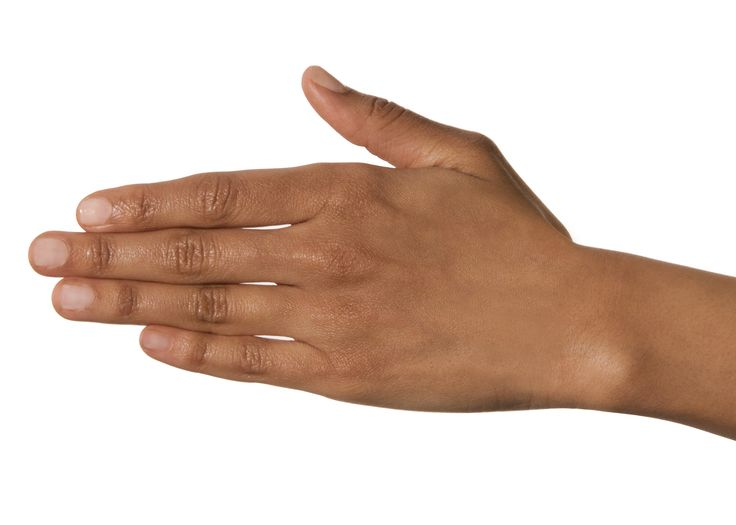
\includegraphics[width=\textwidth,height=\textheight,keepaspectratio]{../inputs/hand_brown.jpg}
  \end{minipage} & 
  \begin{minipage}{.29\textwidth}
    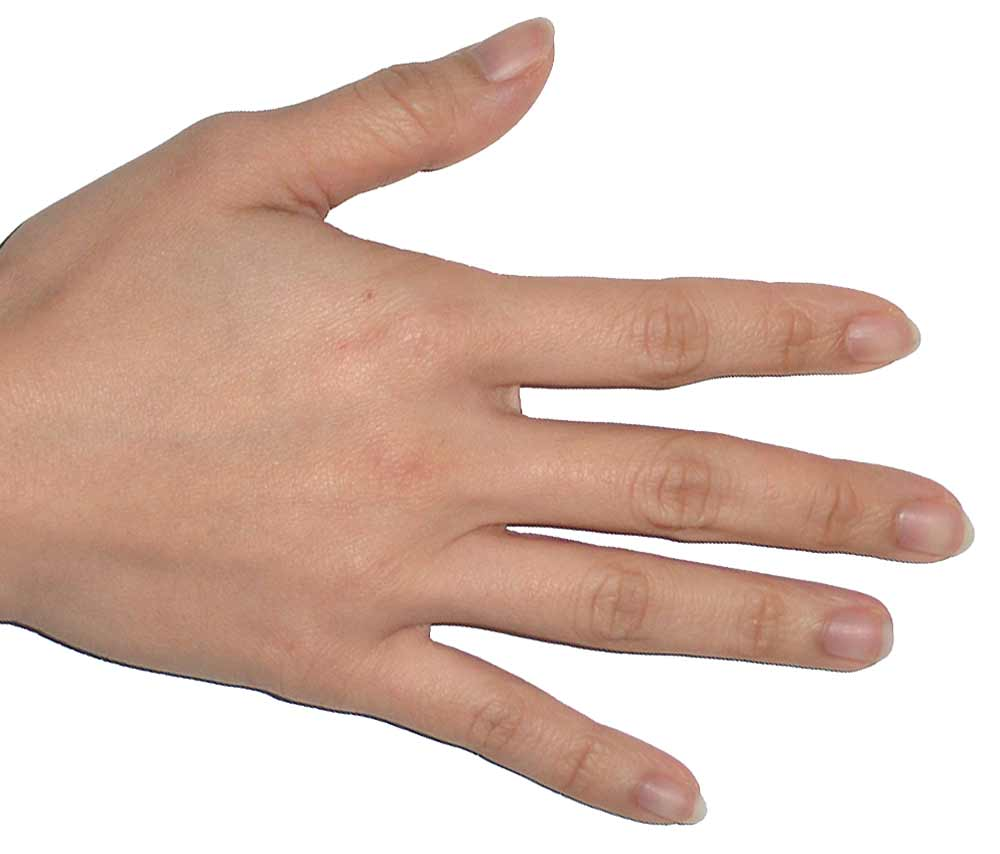
\includegraphics[width=\textwidth,height=\textheight,keepaspectratio]{../inputs/hand_light.jpg}
  \end{minipage} & 
  \begin{minipage}{.29\textwidth}
    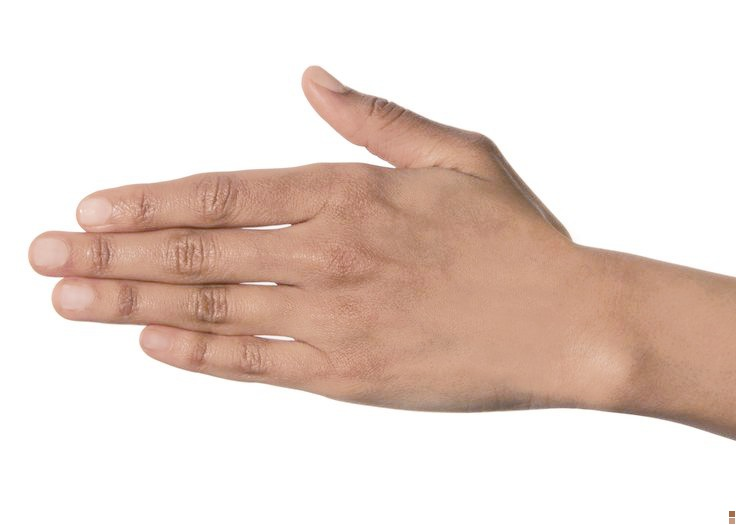
\includegraphics[width=\textwidth,height=\textheight,keepaspectratio]{../rc_test/outputs/20170524_prop_corr_1p1_ave_100/hand_brown_to_hand_light.jpg}
  \end{minipage} \\
\hline
 \end{longtable}

To narrow the scope of our project, we will not include skin detection as part of this project and assume that our algorithm is already given a mask of the skin areas of all the images. We will focus solely on the transfer of the hand skin colour. 

Based on our goals and the nature of our project, we list below several constraints and design paradigms against which we will evaluate our algorithm:

\textbf{Compatibile with mobile device:} Our algorithm is ultimately intended to support and application on a mobile device, so we must ensure that our code is portable to mobile devices and that the algorithm we develop can operate quickly with the limited resources of a mobile device so that the user will be able to see near-instant results.

\textbf{Fully automatic:} Since the goal of our project is for a commercial user to be able to change the model to his or her own skin colour, our algorithm cannot rely on any user input to perform the image editing and should able to accept only an image containing the user's own hand as the target image to transfer the colour of the model hand to.

\textbf{Realistic skin colour transfer:}
Since the goal of our project is to perform skin colour transfer for model images that are meant to demonstrate cosmetic products to users, and the results are meant to invoke for the user the impression that the user's own hand is wearing the product, our final images must look as realistic as possible to avoid a displeasing, uncanny valley effect. Furthermore, the images we process will be large and feature a the skin on the back of a hand very prominently, so we can expect the realistic appearance we can expect that our result will be very heavily scrutinized by the user.

\textbf{Accurate skin colour transfer:} 
Since the entire goal of nail polish try-on application is to demonstrate to the user how a particular shade of nail polish will appear on his or her own hand, we must ensure that the results of the algorithm, more than looking pleasing to the user, actually matches the skin colour sample provided by the user exactly.

\textbf{Wide range of colour transfer:} Since the goal of the project is to reduce the number of nail polish try-on videos of different skin colours needed and since users may have a wide range of skin colour and should all be supported, our algorithm needs to be able to transfer the skin colour of a mid-toned hand to as wide a range of skin colour as possible.

 % use of a target image, , speed of the colour transfer on a mobile device, range of colour transfer